\begin{frame}
  \frametitle{Fact 1 -- Sum of Degrees}
{ \Huge
  \[
    \sum_{u\in V} degree(u) = 2|E|
  \]
}
  Every edge contributes exactly once to the degree of exactly two nodes.
\end{frame}

\begin{frame}
  \frametitle{Fact 2 -- Average Degree}
\begin{equation}
\begin{aligned}
E(degree(X)) & = \sum_{u\in V} Pr(X=u)\cdot degree(u)\\
              & = \frac{1}{n} \sum_u degree(u) = \frac{2|E|}{n}
  \end{aligned}
  \end{equation}
\end{frame}

\begin{frame}
  \frametitle{Fact 3 -- Min-cut Size}

  The size of a min-cut is at most $\frac{2|E|}{n}$.

  \only<1>{ 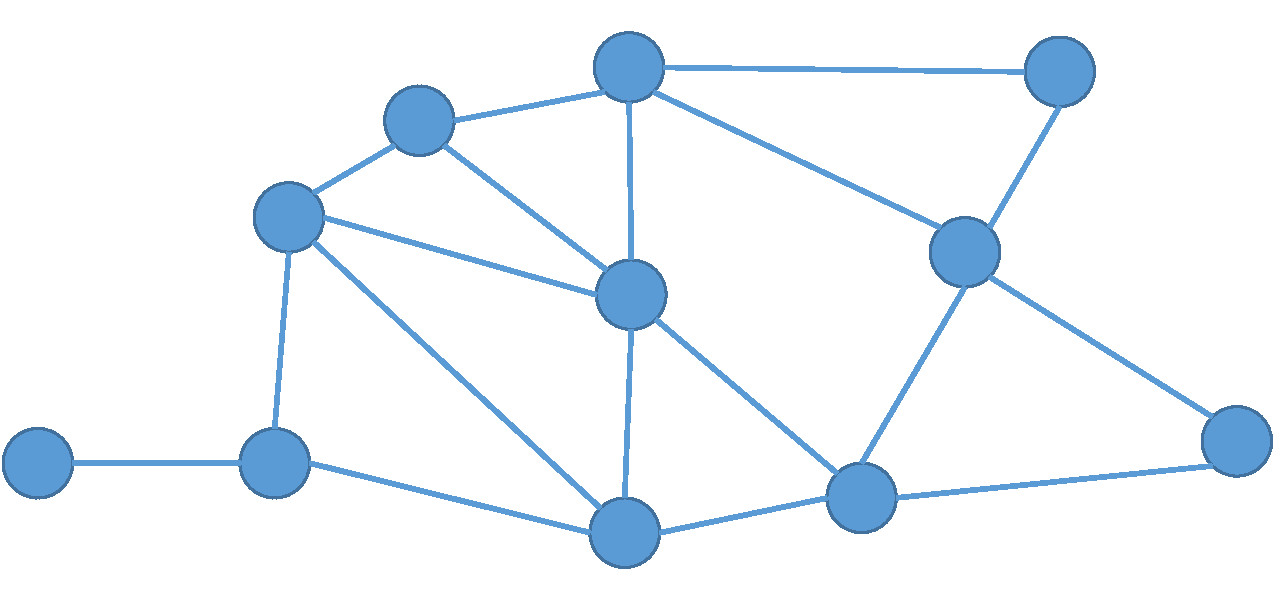
\includegraphics[scale=0.4]{img/fact3_1.pdf} }
  \only<2>{ 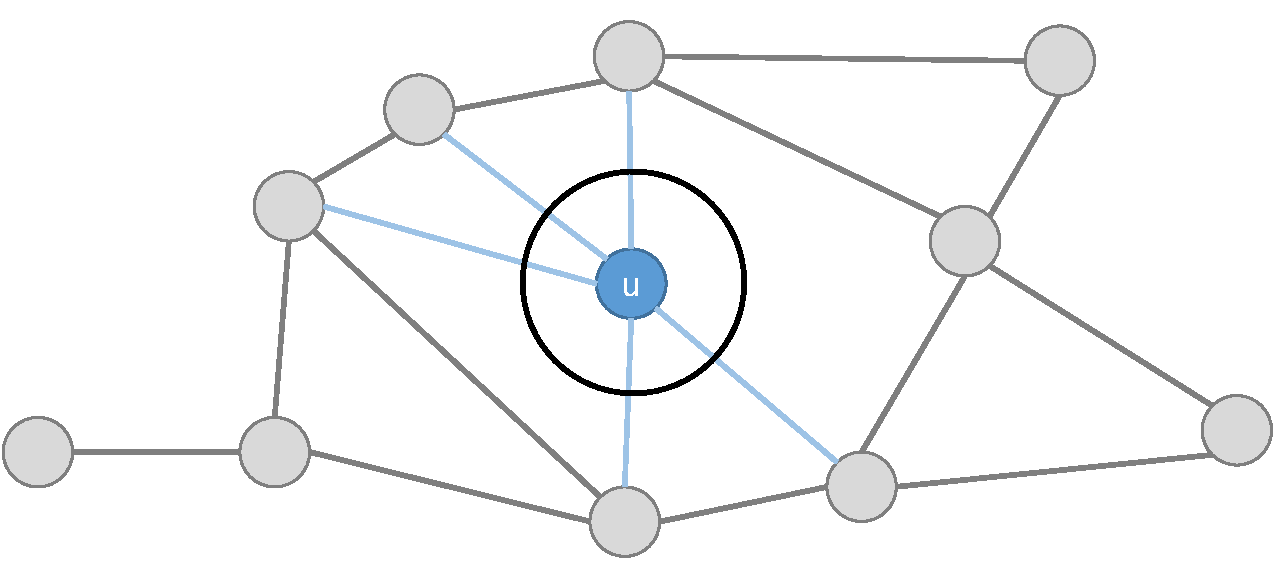
\includegraphics[scale=0.4]{img/fact3_2.pdf} }
  \only<3>{
    \begin{greenblock}{Proof}
      \begin{itemize}
        \item For every node $u$, we have a cut of size $degree(u)$.
        \item Not all nodes can have degree above average, i.e.
      \end{itemize}
      \[
        \exists u\in V:\ degree(u) \leq \frac{2|E|}{n}
      \]
    \end{greenblock}
  }

\end{frame}

\begin{frame}
  \frametitle{Fact 4 -- Pr[edge across min-cut]}

  \begin{itemize}
    \item Fix a certain min-cut in a graph.
    \item At most $2|E|/n$ of all edges are part of this min-cut.
    \item Choose a random edge out of all $|E|$ edges.
    \item $Pr(\text{edge crosses the cut}) = \frac{2|E|/n}{|E|} = \frac{2}{n}$
  \end{itemize}

\end{frame}


\begin{frame}
  \frametitle{Concentrating = Not Cutting}
  \begin{itemize}
  \item {\bf\large TODO} show the running example and explain how an
    edge that has been concentrated will never be cut.
  \item And the edges that remain at the end, because they have never
    been concentrated.
  \end{itemize}
\end{frame}

\begin{frame}
  \frametitle{Success Probability}

\only<1>{
  \begin{itemize}
  \item Fix a certain min-cut
  \item We can never contract an edge from that cut
  \item $Pr[first~edge~is~not~in~min~cut] = 1 - \frac{2}{n}$
  \item Now $n - 1$ edges remaining, so $Pr[second edge is not in min
    cut] = (1 - \frac{2}{n-1})$
  \end{itemize}
}

\only<2>{
  \begin{block}{First Cut is not Fixed Cut }
 \begin{equation*}
    \begin{aligned}
Pr[fi&\left(nal~cut~is~not~the~fixed~cut]\right)\\
   =  &\left(    Pr[no contracted edge is in minimun cut] \right)\\
 \le  & \left(   (1 - \frac{2}{n})(1 - \frac{2}{n-1})(1 - \frac{2}{n-2})...(1 -
   \frac{2}{4})(1 - \frac{2}{3}) \right)\\
  =  &\left(  \frac{n-2}{n} \right)
    \end{aligned}
   \end{equation*}

  \end{block}
}

\only<3>{
  \begin{block}{Series Convere to e}
    \begin{itemize}
    \item $e = \lim(1 + \frac{1}{n})^n$
    \item $\lim(1 + \frac{1}{n})^n = \lim(1 +
      \frac{1}{\frac{n}{a}})^{\frac{n}{a}\cdot a}$
    \item Let $x = \frac{n}{a}$
    \end{itemize}
    $\lim(1 + \frac{1}{n})^n = \lim(1 + \frac{1}{x})^{x\cdot a}$
    $ =( \lim(1 + \frac{1}{x})^x)^a = e^x$
  \end{block}
}

\end{frame}

\begin{frame}
  \frametitle{Boosting Success Probability}

\only<1>{




Assumn that we can get the best result by running the algorithm $k$
times.
\begin{itemize}
\item Probability of at least one success:
$1 - (1 - \frac{1}{\binom{n}{2}})^k$
\item To make it an e-series, we need $k$ to contain $\binom{n}{2}$.
\end{itemize}

Here we can use $a = -1$ and $k = \binom{n}{2}\cdot c\cdot \ln{n}$
Running time is thus promised:
$$O(k)\cdot O(n^2) = O(n^4\log{n})$$

}

\only<2>{
  \begin{equation*}
    \begin{aligned}
1 - (1 - \frac{1}{\binom{n}{2}})^k  &= 1 - (1 +
\frac{1}{\binom{n}{2}})^{-k}\\
& =1 - ((1 + \frac{1}{\binom{n}{2}})^{\binom{n}{2}})^{-c\cdot\ln{n}}\\
& = 1 - e^{-c\cdot\ln{n}} = 1 - (e^{\ln{n}})^{-c}\\
& =1 - \frac{1}{n^c}
    \end{aligned}
  \end{equation*}


}

\only<3>{
The error probability is thus:

$$
O( \frac{1}{n^c})
$$

}
\end{frame}


\begin{frame}
  \frametitle{Extended Karger's Analysis}
One run succeeds with $\Omega(\frac{1}{\log{n}})$. If we run the
algorithm$k = \log^2{n}$ times:
\begin{equation*}
  \begin{aligned}
Pr[at~least~one~run~succeeds] & =1 - (1 - \frac{1}{log{n}})^{\log^2{n}}\\
& = 1 - (1 + \frac{1}{-log{n}})^{-\log{n}\cdot-\log{n}}\\
& =1 -e^{-\log{n}} = 1 - \frac{1}{n} \\
& \Rightarrow Pr[error] O(\frac{1}{n})
  \end{aligned}
\end{equation*}
\end{frame}
